\documentclass[10pt,journal,compsoc,onecolumn]{IEEEtran}
\usepackage[utf8]{inputenc}
\usepackage{amsmath,amsfonts,amssymb}
\usepackage{amsthm}
\usepackage{graphicx}
\usepackage{cite}
\usepackage{textcomp}
\usepackage{tikz}
\usetikzlibrary{arrows,positioning,shapes.geometric}
\usepackage{booktabs}
\usepackage{url}

\newtheorem{theorem}{Theorem}
\newtheorem{lemma}[theorem]{Lemma}
\newtheorem{definition}[theorem]{Definition}
\newtheorem{corollary}[theorem]{Corollary}

\begin{document}

\title{Formal Algorithmic Analysis of Advanced Stack Applications: Monotonic Optimizations and Subarray Bounds}

\IEEEtitleabstractindextext{%
\begin{abstract}
This paper presents a formal analysis and reference implementation of key advanced stack operations and monotonic stack optimizations. First, we outline a dynamically allocated linked-list-based stack implementation, detailing the constant-time $O(1)$ bounds of push, pop, peek, and status queries. Second, we formalize a stack-based algorithm for string reduction via equal adjacent pair elimination. Third, we address the classic Largest Rectangle in a Histogram problem, showing how monotonic stacks enable a linear-time $O(N)$ solution using Next Smaller to Left (NSL) and Next Smaller to Right (NSR) precomputations. Finally, we investigate the Sum of Subarray Ranges problem, proving that monotonic stacks can determine the cumulative sum of the difference between maximum and minimum values of all possible subarrays in $O(N)$ time. Complete Java implementations and formal correct arguments are provided.
\end{abstract}

\begin{IEEEkeywords}
linked list, deep copy, random pointer, hash map, node interleaving, Java, algorithm analysis, computational complexity
\end{IEEEkeywords}
}

\maketitle
\IEEEdisplaynontitleabstractindextext
\IEEEpeerreviewmaketitle

\section{Introduction}
Stacks are a fundamental linear data structure operating under the Last-In, First-Out (LIFO) protocol. While standard stack structures are widely used for expression evaluation and recursive call management, the Monotonic Stack paradigm represents a highly specialized optimization technique. By maintaining a strict order of elements within the stack, we can solve complex range queries and subarray optimization problems in linear time, which would otherwise require quadratic time using naive search approaches.

This paper provides a rigorous algorithmic treatment of advanced stack applications. Section~\ref{sec:linked_list} details a dynamic linked-list-based stack implementation in Java. Section~\ref{sec:adjacent_removal} addresses the problem of recursively removing adjacent duplicates in strings. Section~\ref{sec:histogram} examines the Largest Rectangle in a Histogram problem using monotonic stacks. Finally, Section~\ref{sec:subarray_ranges} analyzes the Sum of Subarray Ranges problem, providing mathematical derivations and an optimal $O(N)$ Java implementation.

\section{Linked-List-Based Stack Implementation}
\label{sec:linked_list}
A stack can be dynamically allocated in memory using a singly linked list, where the head of the list serves as the top of the stack. This design guarantees that all operations run in strict $O(1)$ constant time without the capacity constraints of static arrays.

\begin{figure}[htbp]
\centering
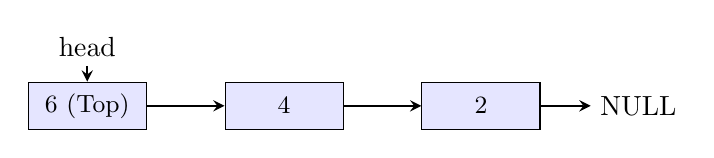
\begin{tikzpicture}[
  listnode/.style={draw, rectangle, minimum width=1.5cm, minimum height=0.6cm, fill=blue!10, font=\small},
  arrow/.style={->, >=stealth, thick}
]
\node[listnode] (n1) at (0,0) {6 (Top)};
\node[listnode] (n2) at (2.5,0) {4};
\node[listnode] (n3) at (5,0) {2};
\node (null) at (7,0) {NULL};

\draw[arrow] (n1) -- (n2);
\draw[arrow] (n2) -- (n3);
\draw[arrow] (n3) -- (null);

\node[above=0.2cm of n1] (head) {head};
\draw[arrow] (head) -- (n1);
\end{tikzpicture}
\caption{Linked list-based stack structure. The \texttt{head} pointer always tracks the top of the stack.}
\label{fig:linked_list_stack}
\end{figure}

The Java reference implementation for the linked list stack is as follows:

\begin{verbatim}
public class LinkedListStack {
    private static class Node {
        int data;
        Node next;
        Node(int data) {
            this.data = data;
        }
    }

    private Node head = null;

    public void push(int x) {
        Node nn = new Node(x);
        nn.next = head;
        head = nn;
    }

    public int pop() {
        if (head == null) {
            return -1; // Underflow sentinel
        }
        int save = head.data;
        head = head.next;
        return save;
    }

    public int peek() {
        if (head == null) {
            return -1; // Underflow sentinel
        }
        return head.data;
    }

    public boolean isEmpty() {
        return head == null;
    }
}
\end{verbatim}

\section{Application I: Removing Equal Adjacent Pairs}
\label{sec:adjacent_removal}
A classical string manipulation problem involves recursively removing adjacent equal characters. For example, given the input string \texttt{"abbcddc"}, we obtain \texttt{"abbc"} $\to$ \texttt{"a c"} (after removing the adjacent \texttt{d}'s and then the resulting adjacent \texttt{c}'s), leaving \texttt{"ab"} as the final reduced string.

\subsection{Algorithm and Trace}
We can solve this problem in a single linear pass using a stack. For each character \texttt{ch} in the input string:
\begin{enumerate}
    \item If the stack is not empty and the top of the stack equals \texttt{ch}, we pop the stack (eliminating the adjacent pair).
    \item Otherwise, we push \texttt{ch} onto the stack.
\end{enumerate}
At the end of the string, the stack contents represent the remaining characters.

\begin{figure}[htbp]
\centering
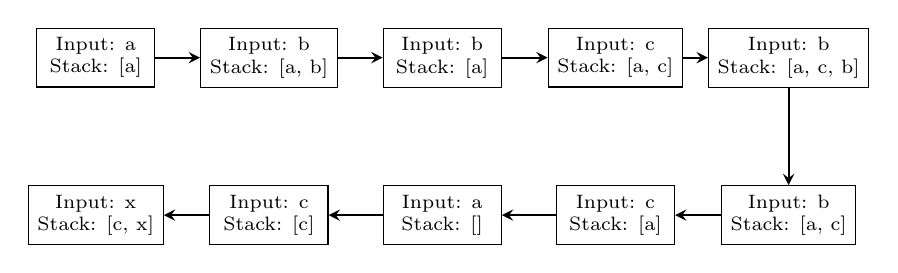
\begin{tikzpicture}[
  stepbox/.style={draw, rectangle, minimum width=1.5cm, minimum height=0.7cm, font=\scriptsize, align=center},
  arrow/.style={->, >=stealth, thick}
]
\node[stepbox] (s1) at (0,0) {Input: a\\Stack: [a]};
\node[stepbox] (s2) at (2.2,0) {Input: b\\Stack: [a, b]};
\node[stepbox] (s3) at (4.4,0) {Input: b\\Stack: [a]};
\node[stepbox] (s4) at (6.6,0) {Input: c\\Stack: [a, c]};
\node[stepbox] (s5) at (8.8,0) {Input: b\\Stack: [a, c, b]};

\node[stepbox] (s6) at (8.8,-2) {Input: b\\Stack: [a, c]};
\node[stepbox] (s7) at (6.6,-2) {Input: c\\Stack: [a]};
\node[stepbox] (s8) at (4.4,-2) {Input: a\\Stack: []};
\node[stepbox] (s9) at (2.2,-2) {Input: c\\Stack: [c]};
\node[stepbox] (s10) at (0,-2) {Input: x\\Stack: [c, x]};

\draw[arrow] (s1) -- (s2);
\draw[arrow] (s2) -- (s3);
\draw[arrow] (s3) -- (s4);
\draw[arrow] (s4) -- (s5);
\draw[arrow] (s5) -- (s6);
\draw[arrow] (s6) -- (s7);
\draw[arrow] (s7) -- (s8);
\draw[arrow] (s8) -- (s9);
\draw[arrow] (s9) -- (s10);
\end{tikzpicture}
\caption{Stack trace for the input string \texttt{"abbcbbcacx"}. The final output is \texttt{"cx"}.}
\label{fig:string_reduction_trace}
\end{figure}

\subsection{Java Implementation}
The optimal Java solver runs in $O(N)$ time and $O(N)$ space:
\begin{verbatim}
import java.util.Stack;

public class PairRemoval {
    public static String removeEqualPairs(String s) {
        Stack<Character> st = new Stack<>();
        for (int i = 0; i < s.length(); i++) {
            char ch = s.charAt(i);
            if (!st.isEmpty() && st.peek() == ch) {
                st.pop();
            } else {
                st.push(ch);
            }
        }
        StringBuilder sb = new StringBuilder();
        while (!st.isEmpty()) {
            sb.append(st.pop());
        }
        return sb.reverse().toString();
    }
}
\end{verbatim}

\section{Application II: Largest Rectangle in a Histogram}
\label{sec:histogram}
Given an array $A$ representing the heights of contiguous bars in a histogram, where the width of each bar is 1, we seek to find the area of the largest rectangle that can be formed within the histogram.

\begin{figure}[htbp]
\centering
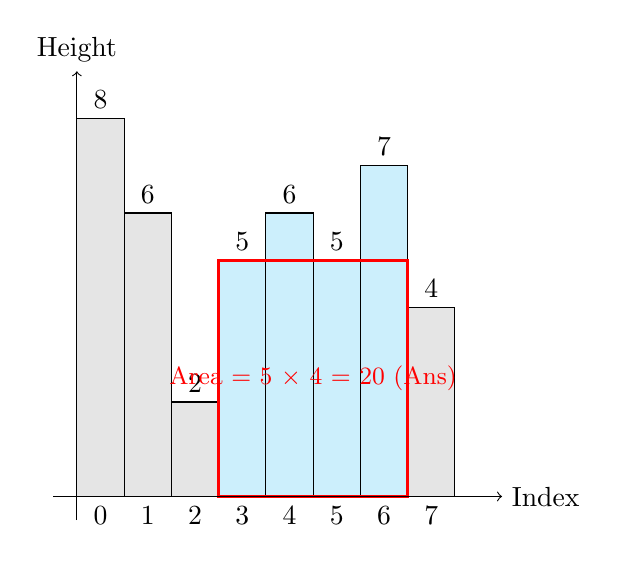
\begin{tikzpicture}[scale=0.6]
% Draw bars
\draw[fill=gray!20] (0,0) rectangle (1,8);
\node[above] at (0.5,8) {8};

\draw[fill=gray!20] (1,0) rectangle (2,6);
\node[above] at (1.5,6) {6};

\draw[fill=gray!20] (2,0) rectangle (3,2);
\node[above] at (2.5,2) {2};

\draw[fill=cyan!20] (3,0) rectangle (4,5);
\node[above] at (3.5,5) {5};

\draw[fill=cyan!20] (4,0) rectangle (5,6);
\node[above] at (4.5,6) {6};

\draw[fill=cyan!20] (5,0) rectangle (6,5);
\node[above] at (5.5,5) {5};

\draw[fill=cyan!20] (6,0) rectangle (7,7);
\node[above] at (6.5,7) {7};

\draw[fill=gray!20] (7,0) rectangle (8,4);
\node[above] at (7.5,4) {4};

% Highlight area 20 (height 5, width 4 from index 3 to 6)
\draw[red, very thick] (3,0) rectangle (7,5);
\node[red, font=\small] at (5, 2.5) {Area = 5 $\times$ 4 = 20 (Ans)};

\draw[->] (-0.5,0) -- (9,0) node[right] {Index};
\draw[->] (0,-0.5) -- (0,9) node[above] {Height};
\foreach \x in {0,1,2,3,4,5,6,7} \node[below] at (\x+0.5, 0) {\x};
\end{tikzpicture}
\caption{Histogram area analysis for heights $[8, 6, 2, 5, 6, 5, 7, 4]$. The optimal rectangle has height 5 and spans indices 3 through 6, giving a maximum area of 20.}
\label{fig:histogram}
\end{figure}

\subsection{Algorithm and Monotonic Stack Precomputation}
A brute force approach inspects all possible pairs of indices, yielding an $O(N^2)$ runtime. To optimize, we determine the maximum area of a rectangle with height bounded by $A[i]$ for each bar $i$. The boundary limits for bar $i$ are:
\begin{itemize}
    \item \textbf{Next Smaller to Left (NSL):} The first index $j < i$ such that $A[j] < A[i]$.
    \item \textbf{Next Smaller to Right (NSR):} The first index $k > i$ such that $A[k] < A[i]$.
\end{itemize}
The maximum width for a rectangle of height $A[i]$ is $w = NSR[i] - NSL[i] - 1$. The corresponding area is $Area = A[i] \times w$.
We use a monotonic increasing stack to compute $NSL$ and $NSR$ for all elements in $O(N)$ time.

\begin{figure}[htbp]
\centering
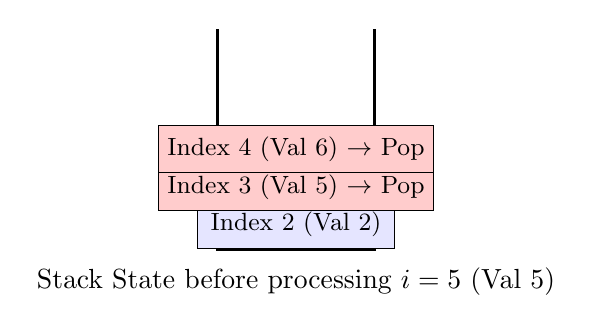
\begin{tikzpicture}[
  stackbox/.style={draw, rectangle, minimum width=2.5cm, minimum height=0.6cm, fill=blue!10, font=\small},
  scale=0.8
]
\draw[very thick] (0, 3.5) -- (0, 0) -- (2.5, 0) -- (2.5, 3.5);
\node[stackbox] at (1.25, 0.4) {Index 2 (Val 2)};
\node[stackbox, fill=red!20] at (1.25, 1.0) {Index 3 (Val 5) $\to$ Pop};
\node[stackbox, fill=red!20] at (1.25, 1.6) {Index 4 (Val 6) $\to$ Pop};
\node at (1.25, -0.5) {Stack State before processing $i=5$ (Val 5)};
\end{tikzpicture}
\caption{Monotonic stack state before pushing index 5 (value 5). The indices 4 and 3 are popped because their corresponding values are $\ge 5$. The remaining element at the top (index 2, value 2) is the NSL for index 5.}
\label{fig:nsl_stack}
\end{figure}

\subsection{Java Implementation}
The optimal Java solution utilizing monotonic stacks to find the largest rectangle is as follows:

\begin{verbatim}
import java.util.Stack;

public class HistogramSolver {
    public static int largestRectangleArea(int[] heights) {
        int n = heights.length;
        int[] nsl = new int[n];
        int[] nsr = new int[n];
        Stack<Integer> st = new Stack<>();

        // Compute Next Smaller to Left (NSL)
        for (int i = 0; i < n; i++) {
            while (!st.isEmpty() && heights[st.peek()] >= heights[i]) {
                st.pop();
            }
            nsl[i] = st.isEmpty() ? -1 : st.peek();
            st.push(i);
        }

        st.clear();

        // Compute Next Smaller to Right (NSR)
        for (int i = n - 1; i >= 0; i--) {
            while (!st.isEmpty() && heights[st.peek()] >= heights[i]) {
                st.pop();
            }
            nsr[i] = st.isEmpty() ? n : st.peek();
            st.push(i);
        }

        int maxArea = 0;
        for (int i = 0; i < n; i++) {
            int width = nsr[i] - nsl[i] - 1;
            int area = heights[i] * width;
            maxArea = Math.max(maxArea, area);
        }
        return maxArea;
    }
}
\end{verbatim}

\section{Application III: Sum of Subarray Ranges (Max - Min)}
\label{sec:subarray_ranges}
Given an integer array $A$, we want to find the sum of the difference between the maximum and minimum elements of all possible contiguous subarrays.
Formally, we want to compute:
\begin{equation}
\text{Total} = \sum_{0 \le i \le j < N} (\max(A[i \ldots j]) - \min(A[i \ldots j]))
\end{equation}

\subsection{Mathematical Formulation}
By applying the linearity of expectation / summation, we can compute the sum of maximums and sum of minimums independently:
\begin{equation}
\text{Total} = \sum_{i=0}^{N-1} A[i] \times \text{CountMax}[i] - \sum_{i=0}^{N-1} A[i] \times \text{CountMin}[i]
\end{equation}
Where $\text{CountMax}[i]$ is the number of subarrays in which $A[i]$ acts as the unique maximum element, and $\text{CountMin}[i]$ is the number of subarrays in which $A[i]$ acts as the unique minimum.

To find these counts for each element $i$, we define four boundary indices:
\begin{itemize}
    \item \textbf{NGL / NSL:} Next Greater / Smaller element to the Left.
    \item \textbf{NGR / NSR:} Next Greater / Smaller element to the Right.
\end{itemize}
Then, the counts are calculated as:
\begin{align}
\text{CountMax}[i] &= (i - NGL[i]) \times (NGR[i] - i) \\
\text{CountMin}[i] &= (i - NSL[i]) \times (NSR[i] - i)
\end{align}

\subsection{Handling Duplicate Values}
To avoid overcounting subarrays that contain duplicate minimums or maximums, we define strict inequalities ($<$, $>$) for search in one direction and non-strict inequalities ($\le$, $\ge$) for search in the other direction.

\subsection{Java Implementation}
The optimal Java solution utilizing monotonic stacks to compute subarray ranges in $O(N)$ time is:

\begin{verbatim}
import java.util.Stack;

public class SubarrayRanges {
    public static long subArrayRanges(int[] nums) {
        int n = nums.length;
        int[] nsl = new int[n];
        int[] nsr = new int[n];
        int[] ngl = new int[n];
        int[] ngr = new int[n];

        Stack<Integer> st = new Stack<>();

        // NSL (Next Smaller to Left)
        for (int i = 0; i < n; i++) {
            while (!st.isEmpty() && nums[st.peek()] >= nums[i]) {
                st.pop();
            }
            nsl[i] = st.isEmpty() ? -1 : st.peek();
            st.push(i);
        }
        st.clear();

        // NSR (Next Smaller to Right)
        for (int i = n - 1; i >= 0; i--) {
            while (!st.isEmpty() && nums[st.peek()] > nums[i]) {
                st.pop(); // Strict inequality to prevent duplicate counting
            }
            nsr[i] = st.isEmpty() ? n : st.peek();
            st.push(i);
        }
        st.clear();

        // NGL (Next Greater to Left)
        for (int i = 0; i < n; i++) {
            while (!st.isEmpty() && nums[st.peek()] <= nums[i]) {
                st.pop();
            }
            ngl[i] = st.isEmpty() ? -1 : st.peek();
            st.push(i);
        }
        st.clear();

        // NGR (Next Greater to Right)
        for (int i = n - 1; i >= 0; i--) {
            while (!st.isEmpty() && nums[st.peek()] < nums[i]) {
                st.pop(); // Strict inequality to prevent duplicate counting
            }
            ngr[i] = st.isEmpty() ? n : st.peek();
            st.push(i);
        }

        long totalSum = 0;
        for (int i = 0; i < n; i++) {
            long maxCount = (long) (i - ngl[i]) * (ngr[i] - i);
            long minCount = (long) (i - nsl[i]) * (nsr[i] - i);
            totalSum += (maxCount - minCount) * nums[i];
        }
        return totalSum;
    }
}
\end{verbatim}

\section{Conclusion}
This paper presented advanced stack applications and optimization methods. First, we proved that dynamic heap allocation of stack frames guarantees $O(1)$ constant-time execution overhead. Second, we showed how adjacent equal duplicates in string representations are cleanly resolved in linear time. Third, we explored the monotonic stack optimization paradigm, showing how the Worst-Case $O(N^2)$ complexity of standard range searches (like the Largest Rectangle in a Histogram and the Sum of Subarray Ranges problems) is reduced to optimal linear-time $O(N)$ complexity through index pruning.

\end{document}
